% \subsection*{Polar Coordinates}
% Displacement-strain relations,
% \begin{gather*}
%     \epsilon_r = \frac{\partial u}{\partial r}, \quad \epsilon_\theta = \frac{u}{r} + \frac{1}{r} \frac{\partial v}{\partial \theta} \\
%     2\epsilon_{r\theta} = \gamma_{r\theta} = \frac{\partial v}{\partial r} - \frac{v}{r} + \frac{1}{r} \frac{\partial u}{\partial \theta}
% \end{gather*}
% Strain-stress relations for plane stress,
% \begin{gather*}
%     \epsilon_r = \frac{1}{E} \left( \sigma_r - \nu \sigma_\theta \right), \quad \epsilon_\theta = \frac{1}{E} \left( \sigma_\theta - \nu \sigma_r \right)
%     \epsilon_{r\theta} = \frac{1}{2G} \tau_{r\theta} \\
% \end{gather*}
% Airy's stress function $\Phi$ relations,
% \begin{gather*}
%     \sigma_r = \frac{1}{r}\frac{\partial \Phi}{\partial r} + \frac{1}{r^2} \frac{\partial^2 \Phi}{\partial \theta^2}, \quad \sigma_\theta = 
%     \frac{\partial^2 \Phi}{\partial r^2} \\
%     \tau_{r\theta} = \frac{1}{r^2}\frac{\partial \Phi}{\partial \theta} - \frac{1}{r}\frac{\partial^2 \Phi}{\partial r \partial \theta}
% \end{gather*}
% Compatibility,
% \begin{gather*}
%     \nabla^2 \Phi = \frac{\partial^2 \Phi}{\partial r^2} + \frac{1}{r} \frac{\partial \Phi}{\partial r} + \frac{1}{r^2} \frac{\partial^2 \Phi}{\partial \theta^2} \\
%     \nabla^4 \Phi = \left(\frac{\partial^2}{\partial r^2} + \frac{1}{r} \frac{\partial}{\partial r} + \frac{1}{r^2} \frac{\partial^2}{\partial \theta^2} \right) 
%     \nabla^2 \Phi=0
% \end{gather*}
\section{}
Show that the case of a concentrated load on a straight boundary (Figure \ref{fig:Q1aProblemDiagram}) is represented by the
stress function
\begin{equation*}
    \Phi = -\frac{P}{\pi} r \theta \sin\theta
\end{equation*}
and derive 
\begin{equation*}
    \sigma_r = - \frac{2P}{\pi} \frac{\cos\theta}{r}, \quad \sigma_\theta = 0, \quad \tau_{r\theta} = 0
\end{equation*}
\begin{figure}[h]
    \centering
    \begin{subfigure}[t]{0.35\linewidth}
        \centering
        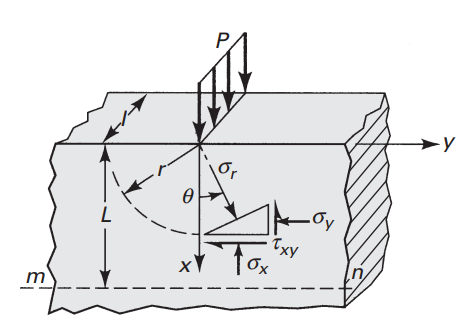
\includegraphics[width=\linewidth]{Questions/Figures/Q1aProblemDiagram.png}
        \caption{Concentrated load on a straight boundary of a large plate}
        \label{fig:Q1aProblemDiagram}
    \end{subfigure}
    \begin{subfigure}[t]{0.35\linewidth}
        \centering
        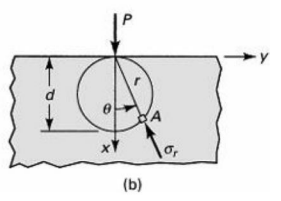
\includegraphics[width=\linewidth]{Questions/Figures/Q1bProblemDiagram.png}
        \caption{Circle of constant radial stress}
        \label{fig:Q1bProblemDiagram}
    \end{subfigure}
    \label{fig:Q1ProblemDiagrams}
\end{figure}

The stress function must satisfy the biharmonic equation
\begin{align*}
    \nabla^4 \Phi &= \left(\frac{\partial^2}{\partial r^2} + \frac{1}{r} \frac{\partial}{\partial r} + \frac{1}{r^2} \frac{\partial^2}{\partial \theta^2} \right)  = 0
\end{align*}
First we calculate partials for $\Phi$,
\begin{align*}
    \frac{\partial \Phi}{\partial r} &= -\frac{P}{\pi} \theta \sin\theta \\
    \frac{\partial^2 \Phi}{\partial r^2} &= 0 \\
    \frac{\partial \Phi}{\partial \theta} &= -\frac{P}{\pi} r \sin\theta - \frac{P}{\pi} r \theta \cos\theta \\
    \frac{\partial^2 \Phi}{\partial \theta^2} &= \frac{P}{\pi}r \theta \sin\theta - \frac{2P}{\pi}r \cos\theta \\
\end{align*}
Next, $\nabla^2 \Phi$ is found by
\begin{align*}
    \nabla^2 \Phi &= \frac{\partial^2 \Phi}{\partial r^2} + \frac{1}{r} \frac{\partial \Phi}{\partial r} + \frac{1}{r^2} \frac{\partial^2 \Phi}{\partial \theta^2}\\
    &=0 + \frac{1}{r} \left(-\frac{P}{\pi} \theta \sin\theta \right) + \frac{1}{r^2} \left(\frac{P}{\pi}r \theta \sin(\theta) 
    - \frac{2P}{\pi}r \cos(\theta) \right) \\
    &= -\frac{P}{\pi} \frac{\theta \sin\theta}{r} + \frac{P}{\pi} \frac{\theta \sin\theta}{r} - \frac{2P}{\pi} \frac{\cos\theta}{r} \\
    &= -\frac{2P}{\pi r} \cos\theta
\end{align*}
Using the result for $\nabla^2 \Phi$ to find partials for $\nabla^4 \Phi$,
\begin{align*}
    \frac{\partial \nabla^2 \Phi}{\partial r} &= \frac{2 P \cos{\theta}}{\pi r^{2}} \\
    \frac{\partial^2 \nabla^2 \Phi}{\partial r^2} &= - \frac{4 P \cos{\theta}}{\pi r^{3}} \\
    \frac{\partial^2 \nabla^2 \Phi}{\partial \theta^2} &= \frac{2 P \cos{\theta}}{\pi r} 
\end{align*}
Finally, for $\nabla^4 \Phi$,
\begin{align*}
    \nabla^4 \Phi &= \left(-\frac{4P\cos\theta}{\pi r^3} \right) + \frac{1}{r} \left(\frac{2P\cos\theta}{\pi r^2} \right) 
    + \frac{1}{r^2} \left( \frac{2P\cos\theta}{\pi r} \right) \\
    &= -\frac{4P\cos\theta}{\pi r^3} + \frac{2P\cos\theta}{\pi r^3} + \frac{2P\cos\theta}{\pi r^3} \\
    &= \boxed{0}
\end{align*}
Therefore, $\Phi$ satisfies the biharmonic equation.

Next, $\sigma_r$ is found by
\begin{align*}
    \sigma_r &= \frac{1}{r} \frac{\partial \Phi}{\partial r} + \frac{1}{r^2} \frac{\partial^2 \Phi}{\partial \theta^2} \\
    &= \frac{1}{r} \left(-\frac{P}{\pi} \theta \sin\theta \right) + \frac{1}{r^2} \left(\frac{P}{\pi}r \theta \sin\theta - \frac{2P}{\pi}r \cos\theta \right) \\
    &= -\frac{P\theta}{\pi r} \sin \theta + \frac{P\theta}{\pi r} \sin \theta - \frac{2P}{\pi r} \cos \theta \\ 
    &= \boxed{-\frac{2P}{\pi r} \cos \theta}
\end{align*}
$\sigma_\theta$ is found by
\begin{align*}
    \sigma_\theta &= \frac{\partial^2 \Phi}{\partial r^2} \\
    &= \boxed{0}
\end{align*}
$\tau_{r\theta}$ is found by
\begin{align*}
    \tau_{r\theta}& =  -\frac{\partial}{\partial r} \left( \frac{1}{r} \frac{\partial \Phi}{\partial \theta} \right) \\
    &= -\frac{\partial}{\partial r} \left( \frac{1}{r} \left(-\frac{P}{\pi} r \sin\theta - \frac{P}{\pi} r \theta \cos\theta \right) \right) \\
    &= -\frac{\partial}{\partial r} \left( -\frac{P}{\pi} \sin\theta - \frac{P}{\pi} \theta \cos\theta \right) \\
    &= \boxed{0}
\end{align*}